% === Begin Label Data ===
% ID: 445
% 难度星级: 
% 标签: 
% 备注: 
% 组卷引用次数: 0
% === End  Label Data ===

\begin{problem}{2017}{G}{上海卷}{12}{解析几何，向量}
如图，用 $35$ 个单位正方形拼成一个矩形，点 $P_1$, $P_2$, $P_3$, $P_4$ 以及四个标记为“$\blacktriangle$”的点在正方形的顶点处，设集合 $\Omega=\{P_1,P_2,P_3,P_4\}$，点 $P\in\Omega$，过 $P$ 作直线 $l_P$，使得不在 $l_P$ 上的“$\blacktriangle$”的点分布在 $l_P$ 的两侧。点 $D_1(l_P)$ 和 $D_2(l_P)$ 分别表示 $l_P$ 一侧和另一侧的“$\blacktriangle$”的点到 $l_P$ 的距离之和。若过 $P$ 的直线 $l_P$ 中有且只有一条满足 $D_1(l_P)=D_2(l_P)$，则 $\Omega$ 中所有这样的 $P$ 为\underline{\hspace{4em}}.

\begin{tikzpicture}[x=0.7cm,y=0.7cm,line cap=round,line join=round]
% grid: 7 columns × 5 rows = 35 unit squares
\draw[step=1,gray!70] (0,0) grid (7,5);
\draw[thick] (0,0) rectangle (7,5);

% points Pi (chosen to match the picture layout)
\fill (0,4) circle (2.2pt) node[left] {$P_1$};
\fill (3,2) circle (2.2pt) node[left] {$P_2$};
\fill (4,2) circle (2.2pt) node[right] {$P_3$};
\fill (6,5) circle (2.2pt) node[above] {$P_4$};

% marked triangle points (▲) at vertices of unit squares
\node at (0,3) {\Large $\blacktriangle$};
\node at (4,4) {\Large $\blacktriangle$};
\node at (1,0) {\Large $\blacktriangle$};
\node at (7,1) {\Large $\blacktriangle$};

% optional: slightly enlarge labels like in the scan
% (remove if you don't want it)
\node[scale=1.6] at ($(0,4)+(0.2,0.1)$) {$\,$};
\end{tikzpicture}
\end{problem}

\begin{answer}
 $P_1,\ P_3,\ P_4$.
\end{answer}

\begin{solutions}
建立平面直角坐标系，如图取四个“$\blacktriangle$”点
$$
A(0,3),\ B(1,0),\ C(7,1),\ D(4,4).
$$
设线段 $AB,BC,CD,DA$ 的中点分别为 $E,F,G,H$，则 $EFGH$ 为平行四边形。

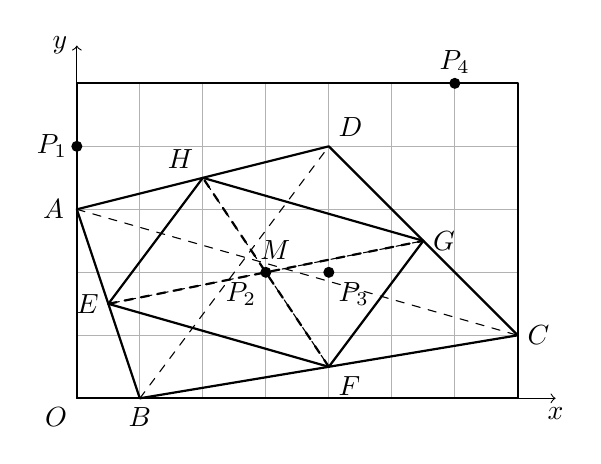
\begin{tikzpicture}[x=0.8cm,y=0.8cm,line cap=round,line join=round]
\usetikzlibrary{calc}

% grid & axes
\draw[step=1,gray!60] (0,0) grid (7,5);
\draw[thick] (0,0) rectangle (7,5);
\draw[->] (0,0) -- (7.6,0) node[below] {$x$};
\draw[->] (0,0) -- (0,5.6) node[left] {$y$};
\node[below left] at (0,0) {$O$};

% ▲ points (given)
\coordinate (A) at (0,3);
\coordinate (B) at (1,0);
\coordinate (C) at (7,1);
\coordinate (D) at (4,4);

% midpoints
\coordinate (E) at ($(A)!0.5!(B)$);
\coordinate (F) at ($(B)!0.5!(C)$);
\coordinate (G) at ($(C)!0.5!(D)$);
\coordinate (H) at ($(D)!0.5!(A)$);

% centroid / intersection
\coordinate (M) at (3,2);

% Ω points (as in the picture layout)
\coordinate (Pone)   at (0,4);   % P1
\coordinate (Ptwo)   at (3,2);   % P2 = M
\coordinate (Pthree) at (4,2);   % P3
\coordinate (Pfour)  at (6,5);   % P4

% quadrilateral ABCD
\draw[thick] (A)--(B)--(C)--(D)--cycle;

% parallelogram EFGH
\draw[thick] (E)--(F)--(G)--(H)--cycle;

% diagonals of EFGH
\draw[dashed,thick] (E)--(G);
\draw[dashed,thick] (F)--(H);

% some auxiliary dashed lines (to mimic the original style)
\draw[dashed] (A)--(C);
\draw[dashed] (B)--(D);
\draw[dashed] (M)--(E) (M)--(F) (M)--(G) (M)--(H);

% marks: ▲
\node at (A) {\Large $\blacktriangle$};
\node at (B) {\Large $\blacktriangle$};
\node at (C) {\Large $\blacktriangle$};
\node at (D) {\Large $\blacktriangle$};

% labels for A,B,C,D,E,F,G,H
\node[left] at ($(A)+(-0.05,0)$) {$A$};
\node[below] at (B) {$B$};
\node[right] at (C) {$C$};
\node[above right] at (D) {$D$};

\node[left] at (E) {$E$};
\node[below right] at (F) {$F$};
\node[right] at (G) {$G$};
\node[above left] at (H) {$H$};

% points P1..P4 (black dots)
\fill (Pone) circle (2.0pt);
\fill (Ptwo) circle (2.0pt);
\fill (Pthree) circle (2.0pt);
\fill (Pfour) circle (2.0pt);

\node[left] at ($(Pone)+(0,0)$) {$P_1$};
\node[below left] at (Ptwo) {$P_2$};
\node[below right] at (Pthree) {$P_3$};
\node[above] at (Pfour) {$P_4$};

\node[above] at ($(M)+(0.15,0.05)$) {$M$};
\node[right] at ($(0,0)+(0.05,0)$) {};
\end{tikzpicture}

设四边形 $ABCD$ 的重心为 $M(x,y)$，则向量恒等式$\overrightarrow{MA}+\overrightarrow{MB}+\overrightarrow{MC}+\overrightarrow{MD}=\vec 0$,

等价于$M=\dfrac{A+B+C+D}{4}=\left(\dfrac{0+1+7+4}{4}, \dfrac{3+0+1+4}{4}\right)=(3,2)$.

而平行四边形 $EFGH$ 的两条对角线交点正是
$\dfrac{E+G}{2}=\dfrac{F+H}{2}=\dfrac{A+B+C+D}{4}=M$,

故该交点即为题设所记的 $P_2$.

对任意过 $P$ 的直线 $l_p$，记 $D_1(l_p),D_2(l_p)$ 为直线两侧（不含直线本身）“$\blacktriangle$”点的个数。
当且仅当 $l_p$ 经过 $P_2$ 时，才能使两侧点数相等（均为 $2$ 个），因此满足条件的直线必过 $P_2$.

于是题意转化为：在 $\Omega=\{P_1,P_2,P_3,P_4\}$ 中，哪些点 $P$ 使得过 $P$ 且过 $P_2$ 的直线唯一。
显然 $P=P_2$ 时过 $P_2$ 的直线无穷多条，不满足“有且仅有一条”。

而 $P_1,P_3,P_4$ 分别与 $P_2$ 确定唯一一条直线，故满足条件的点为 $P_1,\ P_3,\ P_4$.
\end{solutions}